\documentclass[12pt]{article}
\usepackage{graphicx}
\usepackage{amsfonts}
\usepackage{amssymb}
\usepackage{mathrsfs}
\usepackage{amsmath}
\usepackage{algorithm2e}
\usepackage{float}
\usepackage[caption = false]{subfig}
\SetKwInOut{Parameter}{parameter}

\usepackage{enumitem}
\textheight 225mm
\textwidth 166mm
\oddsidemargin 0mm
\evensidemargin 0mm
\topmargin -14mm
\parindent 20pt
\pagestyle{plain}
\pagenumbering{arabic}
\renewcommand{\baselinestretch}{1.18}

\usepackage[unicode]{hyperref}
%\usepackage[numbers,sort&compress]{natbib}
\usepackage{booktabs}
% With this package you can set the size of the margins manually:
\usepackage[margin=1in]{geometry}
\usepackage{amssymb}

%\newenvironment{claim}[1]{\par\noindent\underline{Claim:}\space#1}{}
%\newenvironment{claimproof}[1]{\par\noindent\underline{Proof:}\space#1}{\hfill $\blacksquare$}
\usepackage[hyperref,amsmath, thmmarks]{ntheorem}
\usepackage{mathtools}
\DeclarePairedDelimiter\ceil{\lceil}{\rceil}
\DeclarePairedDelimiter\floor{\lfloor}{\rfloor}

\newtheorem{claim}{Claim}
\theoremsymbol{\rule{1ex}{1ex}}
\newtheorem{proof}{Proof}
\theoremsymbol{\rule{1ex}{1ex}}
\newtheorem{claimproof}{Proof of claim}
\title{Roomba}

\author{Yuhao Zhang}

\date{\today}
\begin{document}
\maketitle
% Enter the exercise number, your name and date here:
%\noindent\parbox{\linewidth}{
% \parbox{.25\linewidth}{ \large HW2 }\hfill
% \parbox{.5\linewidth}{\begin{center} \large Yuhao Zhang \end{center}}\hfill
% \parbox{.2\linewidth}{\begin{flushright} \large Jan 22, 2018 \end{flushright}}
%}
%\noindent\rule{\linewidth}{2pt}


%\section{Introduction}
%
%Briefly introduce the problem here. Describe what you have to do and what the goal is. Make sure to cite any references that you might use \cite{knuth}.
\section{Introduction}
The project is an implementation of a roomba-like system on Sunfounder's PiCar-V platform and a webcam attached to it is used. With the help of QR codes as landmarks, the webcam is turned into a distance-bearing sensor.
\section{Architecheture}
\label{arch}
This project is be based on hierarchical architecture. Though it is a rather early and awkward architecture especially for dynamic world, since it emphasizes on constructing a detailed world model and then carefully planning the action, it is still suitable for PiCar-V and turning it into a Roomba. The reason is that the robot platform used in this project does not equip any sonar/distance sensor, which makes a reactive architecture such as subsumption difficult to realize. We will rely on a pre-constructed world model(or construed through SLAM) and focus on the planning part, as the sense of the robot is rather weak. Therefore the robot will only have static avoidance functionality. The control flow of the system is depicted as Fig.(\ref{cf}).

\begin{figure}[htbp]
\centering
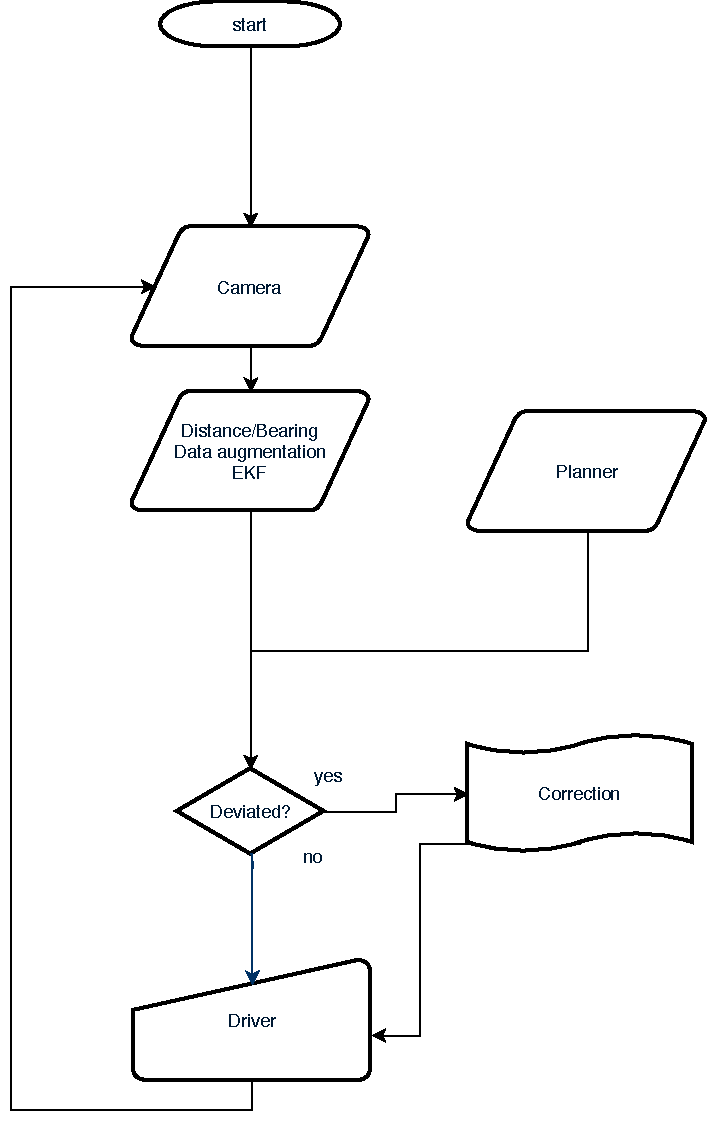
\includegraphics[width=0.5\textwidth]{../figs/cf.pdf}
\caption{The control flow the system}\label{cf}
\end{figure}

\section{Planner}
\label{plan}
The Boustrophedon cellular decomposition is utilized as the planner, please check the referred paper for details. The Boustrophedon cellular decomposition is a variance of trapezoidal decomposition in the sense of dividing the world into cells based on the shape and position of obstacles. Between cells, a usual graph traversal algorithm can be used to determine the route, and within cells, Boustrophedon paths will be generated for the local coverage. An example of such path is shown in Fig.(\ref{bp}).
\begin{figure}[htbp]
\centering
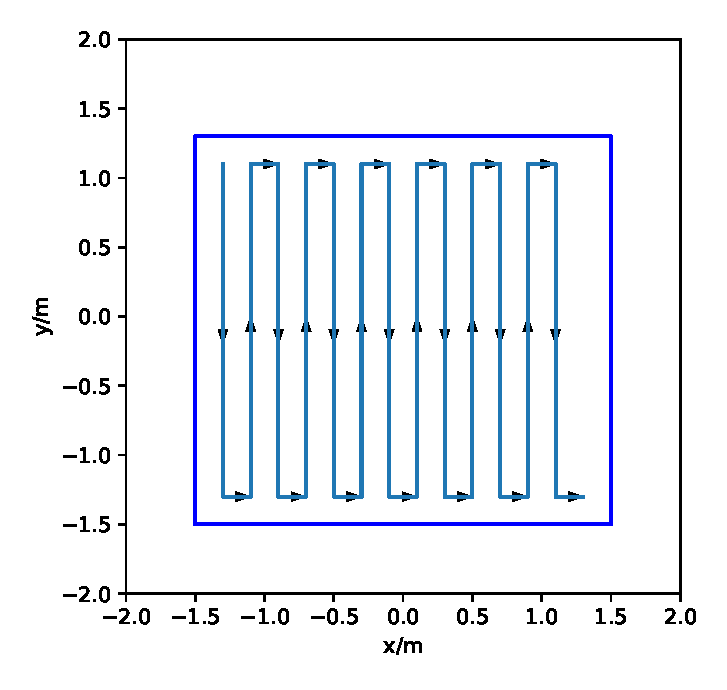
\includegraphics[width=0.6\textwidth]{../figs/bp.eps}
\caption{The Boustrophedon path generated within a rectangular cell}\label{bp}
\end{figure}
\section{Coverage guarantee}
Given that the localization is perfect and the robot can precisely move along the generated trajectory, the Boustrophedon cellular decomposition provides perfect coverage, since it is an exact decomposition of the 2-D plane and inside each cell the cell can be covered perfectly. 

With uncertainty in the system, it becomes trickier to estimate the coverage. Given the error of the localization as $\epsilon$ and assume it is equal to the uncertainty of the motion of the robot. Assuming the width of the cell is $W$ and the width of the robot to be $w$. With the uncertainty the effective width becomes $w\pm \epsilon$. Then the generated Boustrophedon path would have total length 
$$L=W/w\times W.$$ Therefore the total uncertainty of the coverage is $W/w\times W *\epsilon$, which means the ratio of coverage is: 

$$w/\epsilon.$$




\section{Localization}
\label{EKF}
To further improve the performance of the planning, localization of the mobile car can be incorporated.
One major problem for Sunfounder's PiCar-V platform is the lack of a distance-bearing sensor that would make localization with landmarks much easier. However, with the help of known-sized QR tags as 3D object, it is plausible to convert a plain webcam into a distance-bearing sensor.
\subsection{Distance and Pose estimation using PnP}
\label{PnP}
\label{pose}
With a simple pinhole model the scene view $s$ of a camera is formulated as:
$$
s
\begin{pmatrix}
u \\
v \\
1 \\
\end{pmatrix}
=
\begin{pmatrix}
f_x & 0 & c_x \\
0  & f_y &c_y \\
0 & 0 & 1\\
\end{pmatrix}
\begin{pmatrix}
r_{11} & r_{12} & r_{13} & t_1\\
r_{21}  & r_{22} &c_{23} & t_2\\
r_{31} & r_{32} & r_{33} & t_3\\
\end{pmatrix}
\begin{pmatrix}
X \\
Y\\
Z \\
1\\
\end{pmatrix},
$$
where $(X,Y,Z)$ is the coordinate of the object point in world reference frame, $(u,v)$ is the coordinates of the projected object on the view. The first factor on the right hand side is the camera matrix which depicts the intrinsic properties of the camera, while the second factor is the rotation-translation matrix that transforms from world reference frame to the camera frame.

The rotation-translation matrix $R-T$ is solvable by first, detecting the QR code using library such as \texttt{zbar}. Second,  finding the corner points of it and associate with their projections on the view. Once $R-T$ is obtained, one can solve directly for its inverse, as the inverse serves directly for pose estimation of the camera. 

Given $R$ which is the rotation matrix, the inverse of it is denoted as $R^{-1}=R^{T}$. Then the coordinates of the camera in world reference frame are obtained as 

$$(x,y,z)=-R^T V.$$
And the distance between the camera and the object:

$$d=\sqrt{(X-x)^2+(Y-y)^2+Z-z)^2}.$$
Furthermore, the Euler angles representation can also be acquired easily form $R$. As for car-like mobile robots, the motion is usually confined to 2-D plane. Consider such a plane is depicted is a right-hand coordinate system as $x-z$ plane and axis $y$ is pointing to the ground.  Then only Euler angle $ \theta_y$ is of interest. Then the problem can be largely simplified.  For a landmark $M(X,Y,\gamma)$ in world reference frame, the current pose of the camera is 

$$(X-d\cos(\theta_y),Y+d\sin(\theta_y),\pi/2-\theta_y+\gamma).$$
\subsection{Bearing}
The bearing of the object with respect to the camera can be calculated directly using the rotation-translation matrix $R-T$. But in the experiments such calculation turns out to be quite inaccurate and is not sufficient for real application. Therefore in the rest of the paper the bearing is obtained as $$(c_x-c_c)\times \frac{d}{f_x},$$

where $c_x$ is the $x$ principle point as shown in the camera matrix, $c_c$ is the center of the QR tag in camera frame and $f_x$ is the $x-$direction focal length of the camera.

With this pose estimation, one can combine a control algorithm with feedback from QR codes detected by camera.

A picture showing the performance of such model is plotted as  Fig. (\ref{QR}).\begin{figure}[htbp]
\centering
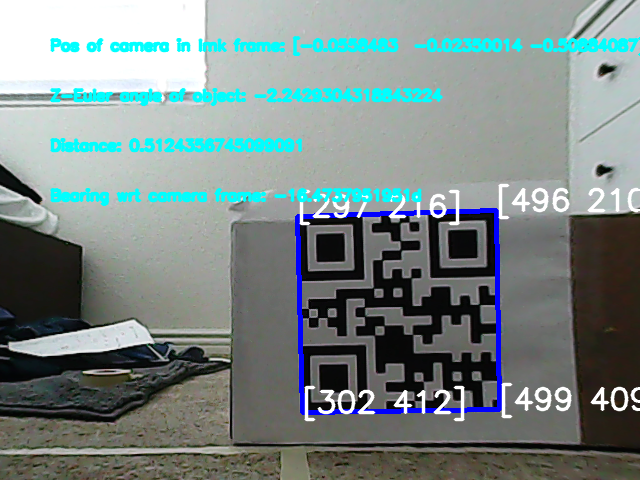
\includegraphics[width=0.6\textwidth]{../figs/bearing_distance.png}
\caption{The QR code used as a landmark.}\label{QR}
\end{figure}

\subsection{EKF}
To utilize the distance-bearing data of the camera, EKF is used for localization.  For initialization, there are 
$$
\bar x =\begin{pmatrix}
x \\
y\\
\theta \\
\end{pmatrix},
P=
\begin{pmatrix}
0 & 0 & 0 \\
0  & 0 &0 \\
0 & 0 & 0 \\
\end{pmatrix}
$$,
where $\bar x$ is the mean vector of robot pose, and $P$ is the covariance matrix. Define the control vector to be $u$, and the perturbation vector to be $n$, one has a generic time-update function:
$$
x \leftarrow f(x,u,n)
$$,
and the EKF prediction:
$$
\bar x \leftarrow f(\bar x, u, 0),
$$
$$
P \leftarrow F_xPF_x^T+F_nNF_n^T,
$$ 
where $F_x$ is the Jacobian of $f(\bar x, u)$ and $F_x$ is the Jacobian of $f(\bar x, n)$.
Further, the observation of land marks can be expressed as an observation function:
$$
y=h(x)+v,
$$
 where $y$ is the actual measurement, $h$ is the observation function and $v$ is the noise. Then the EKF correction can be written as 
 $$
 \bar z = y- h(\bar x)
 $$
 
 $$
  Z=H_xPH
 $$
 
 $$  
 K=PH_x^TZ^{-1}
$$

$$
\bar x \leftarrow +K \bar z
$$

$$
P \leftarrow P-KZK^T,
$$

where $H_x$ is the Jacobian of $h(x)$ and $R$ is the covariance matrix of the measurement noise, $\bar z$ is the innovation mean and $Z$ is the corresponding covariance matrix. $K$ is the Kalman gain.

\section{Kinematics and control law}
\label{kine}
The kinematics of the car is orthogonal to the current 
Ackerman model can be used to describe the kinematics of a car-like robot: 
$$\frac{d x}{dt}=v\cos \theta,$$
$$\frac{d y}{dt}=v\cos \theta,$$
$$\frac{d \theta}{dt}=\frac{v}{L}\tan \gamma,$$
where $(x,y)$ is the position of the middle point of the back wheel axis of the robot in world reference frame. $\theta$ is the angle of pose of the robot. The steering wheel angle is $\gamma$ and the velocity of the back wheel is $v$. $L$ is the length of the vehicle or wheel base.

These equations can be re-written as:
$$
\begin{pmatrix}
\frac{d x}{dt} \\
\frac{d \omega}{dt} \\
\frac{d \theta}{dt} \\
\end{pmatrix}
=
\begin{pmatrix}
\cos \theta & 0 \\
\sin \theta & 0 \\
0 & 1\\
\end{pmatrix}
\begin{pmatrix}
v \\
\omega
\end{pmatrix}.
$$
With the initial position-pose $(x,y,\theta)$ and the goal $(x^*,y^*,\theta^*)$, it is more convenient to write the equations in polar system via a transformation:
$$\rho=\sqrt{\Delta_x^2+\Delta_y^2},$$
$$\alpha=\arctan \frac{\Delta_y}{\Delta_x}-\theta,$$
$$\beta=-\theta-\alpha+\theta^*.$$

The linear control law for $-\pi/2<\alpha\le \pi/2$, i.e. the waypoint is in front of the vehicle is:
$$v=k_\rho \rho,$$
$$\omega=k_\alpha \alpha+k_\beta \beta,$$
where $k_\rho$, $k_\alpha$, $k_\beta$ are arbitrary coefficients that satisfies $k_\rho>0, k_\beta<0,k_\alpha-k_\rho>0.$

The control law for the cases where the waypoint is behind the vehicle is the same as above, but with transformed angles:

$$\alpha'=-\pi-\beta,$$
$$\beta'=-\pi-\alpha,$$
and $v'=-v$.

%\section{Pose estimation}
%\label{pose}
%Without the feedback from sensors, it is required to estimate the motion from the kinematics of the robot directly. Using the linear approximation of the kinematics equations for a short time period $\Delta t$ one can obtain
%$$\Delta(x,y,\theta)=(v\cos \theta \Delta t ,v \sin \theta \Delta t, v/L \tan \gamma \Delta t).$$
%
%Alternatively, the exact solution can be obtained by solving these differential equations directly:
%$$\Delta(x,y,\theta)=(R_b\sin(K\Delta t),R_b(1-\cos(K\Delta t)),K\Delta t),$$
%where $R_b=L/\tan \gamma$ and $K=v/R_b$. However, this estimation is non-linear and makes the control law purposed unstable. Therefore the linear approximation will be used in the following sections.


\section{implementation and setup}
The EKF localization system purposed in Sec.(\ref{EKF}) is implemented in \texttt{EKF-Localization-QRDB.ipynb}. The planner purposed in Sec.(\ref{EKF}) is implemented in \texttt{coverage.ipynb}. The actual setup of the surroundings and the planned path is plotted as Fig.(\ref{vis}).

\begin{figure}[htbp]
\centering

\includegraphics[width=0.6\textwidth]{../figs/visibility_graph_planning.eps}
\caption{The actual setup of the surroundings}\label{vis}
\end{figure}

\begin{figure}[htbp]
\centering
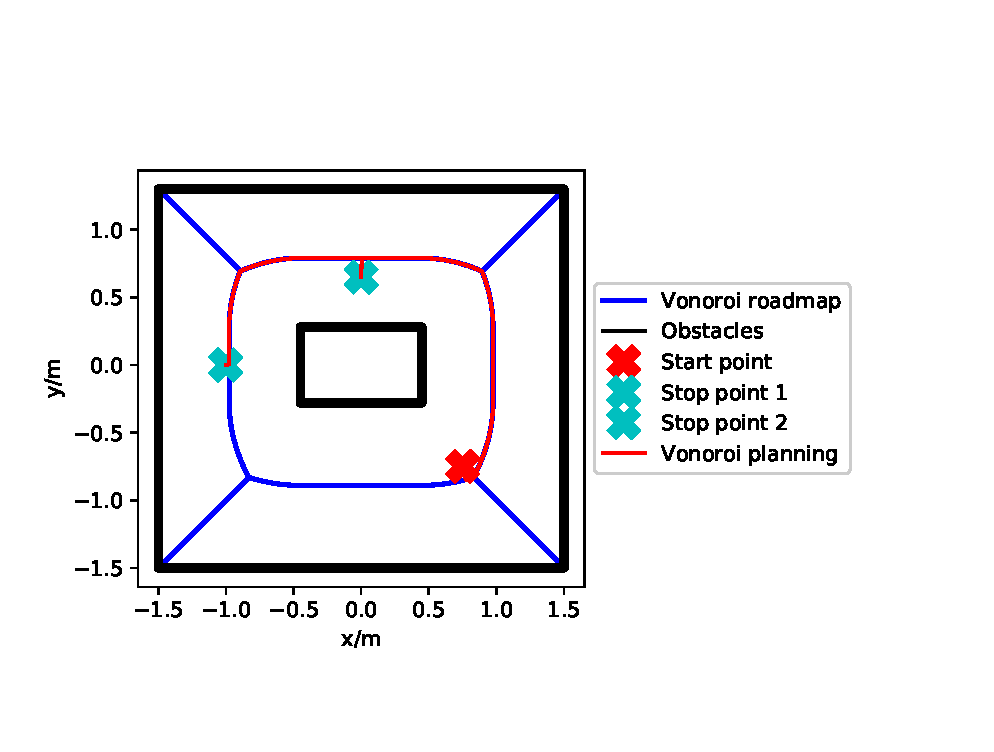
\includegraphics[width=0.6\textwidth]{../figs/vonoroi_planning.eps}
\caption{The actual setup of the surroundings and the planned path by Vonoroi graph planner}\label{vo}
\end{figure}

As of the controller of the robot, one can apply a time-sample linear controller together with an EKF based localization system with the QR tags. Yet for the sake of simplicity, in this project a straight line and constant turning controller is used. Furthermore, it turns out to be nearly impossible to maneuver PiCar-V along a complex 
Boustrophedon path, for the cornering radius of the robot is more than 0.5m, which means the robot is almost incapable of any tiny motion with distance smaller than 0.5m.

\section{Experiment and conclusion}
A movie demonstrating  the performance has been included

The EKF localization system has decent performance(~10 cm error), yet it is very hard to ensure there is always a QR tag in sight to ensure the EKF can be updated in time. Especially when turning at the corner of the planned path, 
The actual performance of the two planners are shown in Tab.(\ref{tab1}). 
\begin{table}[hp]
\centering
\caption{Experiment results}
\label{tab1}
\begin{tabular}{lllr}

Way points    & Planner & Error (m) & Drive time(s)\\
\hline
Strat point      & Visibility graph    & $- $ &-   \\
          & Vonoroi graph        & $- $ &-     \\
Stop point 1       & Visibility graph     & $0.1 \pm 0.05$ &    6.45 \\
		& Vonoroi graph     &$0.1 \pm 0.05$ &     7.50\\
Stop point 2         & Visibility graph     & $0.15 \pm 0.05$    &3.00 \\
		 & Vonoroi graph      & $0.2 \pm 0.05$   &    4.5\\
\hline
\end{tabular}
\end{table}
It can be seen that the two planner performs no difference in terms of the driving accuracy. But the route provided by visibility graph planner is much faster than the path produced by Vonoroi graph planner. As the visibility graph planner tends to give dangerous yet optimal path, while the Vonoroi graph planner gives safe yet conservative path, in experiment the robot runs into the obstacle in about $30\%$ of all runs, and the Vonoroi graph planner never drives the robot into collision. The runs that collides with the obstacle are not taken into account in statistics. 

The conclusion is visibility graph is for optimal path but poses higher risk of collision, and Vonoroi graph planner yields reliable yet slow route. It depends on the task requirement to decide which one is best suitable.
%\begin{figure}[h]
%\subfloat[step 1]{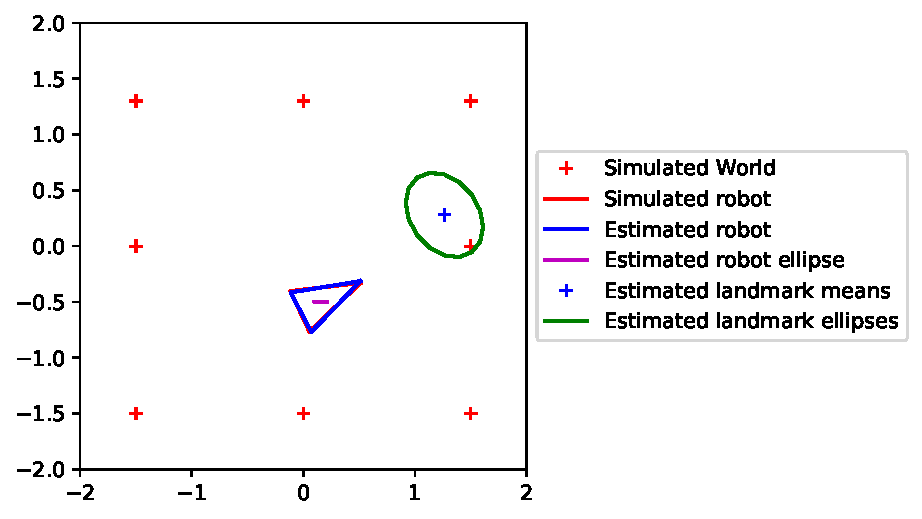
\includegraphics[width = 3in]{./figs/20180514-044756/0.pdf}} 
%\subfloat[step 5]{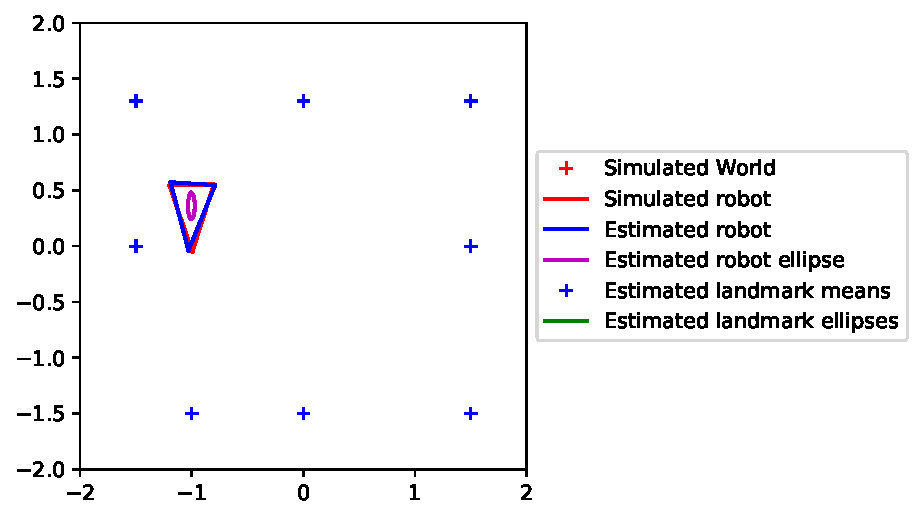
\includegraphics[width = 3in]{./figs/20180514-044756/5.pdf}}\\
%\subfloat[step 10]{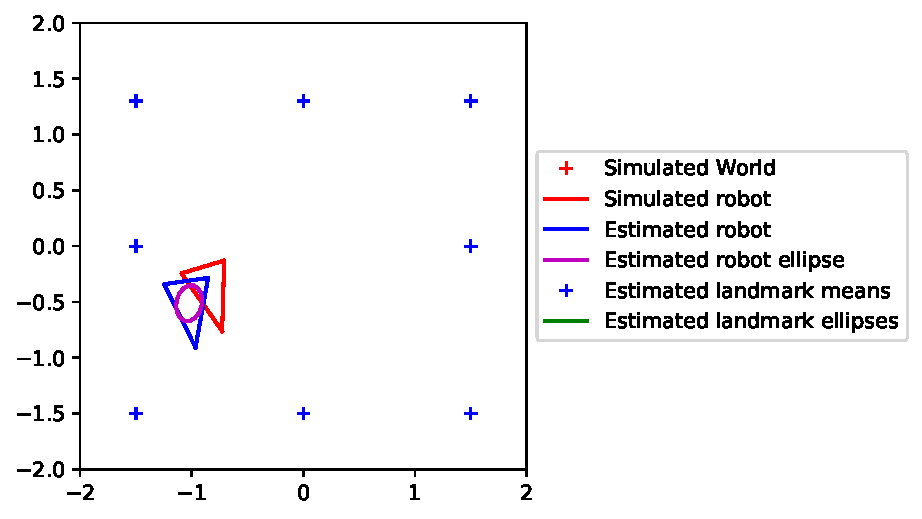
\includegraphics[width = 3in]{./figs/20180514-044756/10.pdf}}
%\subfloat[step 15]{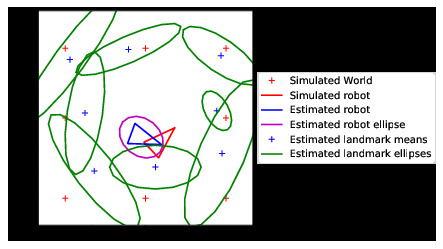
\includegraphics[width = 3in]{./figs/20180514-044756/15.pdf}} \\
%\subfloat[step 20]{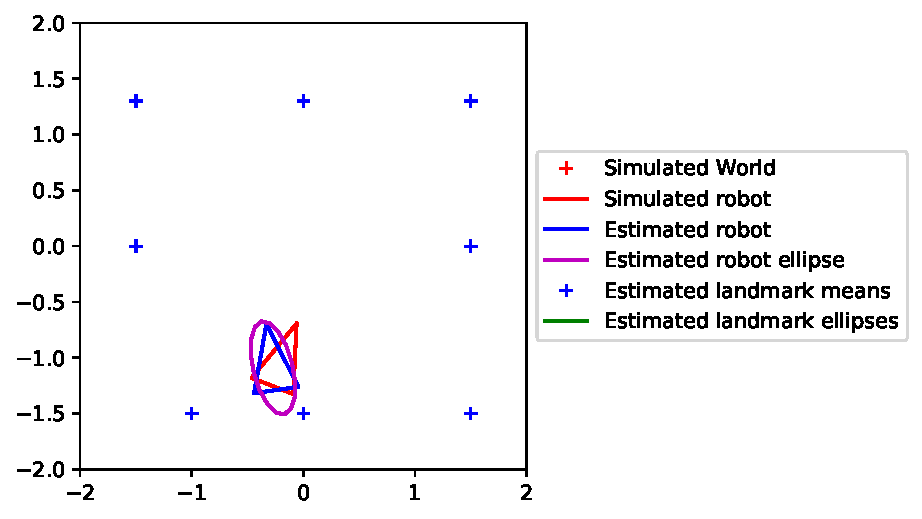
\includegraphics[width = 3in]{./figs/20180514-044756/20.pdf}} 
%\subfloat[step 30]{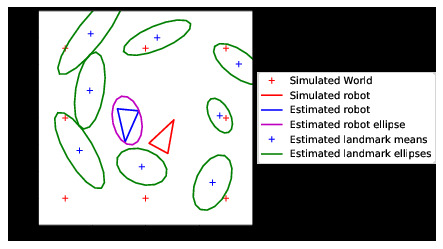
\includegraphics[width = 3in]{./figs/20180514-044756/30.pdf}} \\
%\subfloat[step 50]{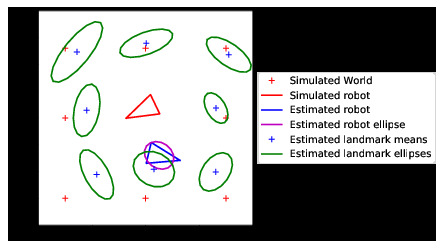
\includegraphics[width = 3in]{./figs/20180514-044756/50.pdf}} 
%\subfloat[step 145]{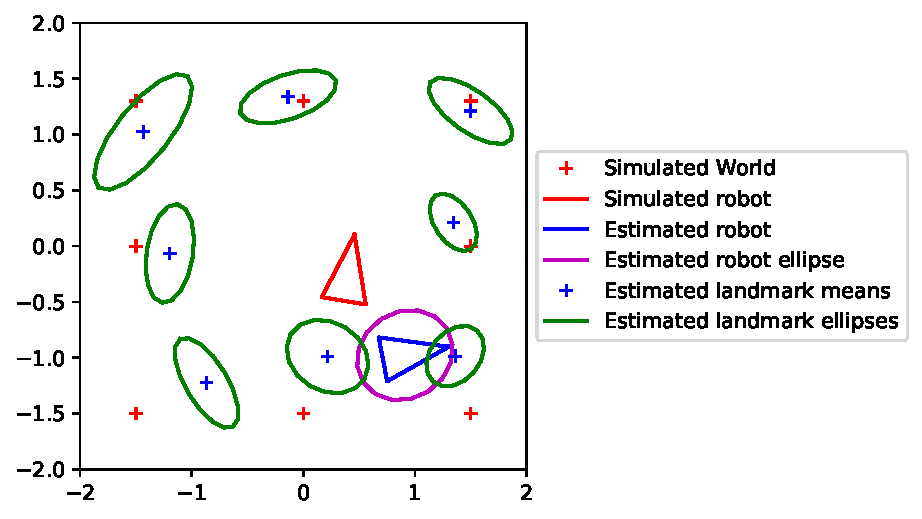
\includegraphics[width = 3in]{./figs/20180514-044756/145.pdf}} \\
%\caption{Intermediate maps as EKF-SLAM goes on. Data entry denoted as \textit{Simulated} means the optimal situation and \textit{Estimated} means the actual data feedback from the sensor and processed with Kalman filter.}
%\label{some}
%\end{figure}


%To see the results of the full run, please check \texttt{ani.gif}.


 

%\clearpage
%\begin{thebibliography}{9}
%
%\bibitem{ekf} 
%Joan Sol\`a: Simulataneous localization and mapping
%with the extended Kalman filter, retrieved at 05-13-2018,
%\\\texttt{http://www.iri.upc.edu/people/jsola/JoanSola/objectes/...\\curs\_SLAM/SLAM2D/SLAM\%20course.pdf}
%\end{thebibliography}
%
%
 
\end{document}



%\begin{figure}[htbp]
%\centering
%\includegraphics[width=0.5\textwidth]{./src/lctwomethods.eps}
%\caption{Learning curve for steepest-direction coordinate descent and random-feature coordinate descent.}\label{fig1}
%\end{figure}









%\subsection{Task 3}
%For 1000 different 100$\times$100 lattices with different $p$ values, the shortest path and the life time of fire is plotted in Fig.(\ref{fig3}). It can be seen clearly that the curves have a phase change point at $p_c\approx0.59$, after which the minimal step and life of fire drop quickly and approximates 100, the width of lattice.
%
%\begin{figure}[htbp]
%\centering
%\includegraphics[width=0.5\textwidth]{../figures/N100pvariable.eps}
%\caption{1000 different 100$\times$100 lattices with different $p$ values, the shortest path and the life time of fire}\label{fig3}
%\end{figure}
%
%For different values of width of lattice $N$, we use 1000 different random lattices per $N$ to find the correlation between the ratio of spanning cluster and the $p$ value, which is plotted in Fig.(\ref{fig4})
%
%
%\begin{figure}[htbp]
%\centering
%\includegraphics[width=0.5\textwidth]{../figures/ratio.eps}
%\caption{1000 different lattices of $N=50, 100, 200$ with different $p$ values, the ratio of the spanning cluster}\label{fig4}
%\end{figure}
%
%
%\section{Discussion}
%It can be found through these figures that $p_c\approx0.59$ and it is irrelevant to the width of lattice $N$.
%\begin{thebibliography}{99}
%
%\bibitem{knuth}
%  Knuth, Ervin D.,
%  \emph{The art of computer programming}, 
%  Addison Wesley, Massachusetts,
%  3rd edition,
%  1997.
%
%\end{thebibliography}

\end{document}